\documentclass[aps, prb, twocolumn, superscriptaddress, amsmath, amssymb]{revtex4-2}

\usepackage{graphicx}
\usepackage{lipsum}
% \usepackage{bm}

\begin{document}

\title{Example of an article with vector and raster images}

\author{C. W. Galdino}
\affiliation{``Gleb Wataghin'' Institute of Physics, University of Campinas (UNICAMP), Campinas, S\~ao Paulo, 13083-859, Brazil}


\date{\today}

\begin{abstract}
\lipsum[1]
\end{abstract}

\maketitle

\section{Introduction}

\lipsum[1]




\section{Vector images}
\lipsum[3]

\begin{figure}
	\centering
	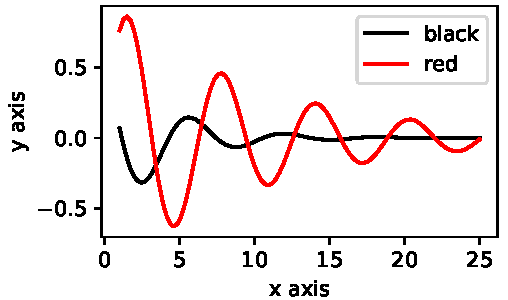
\includegraphics{vector_solid}
	\caption{Example of a vector image with solid lines.}
	\label{vector_solid}
\end{figure}

\lipsum[4]

\begin{figure}
	\centering
	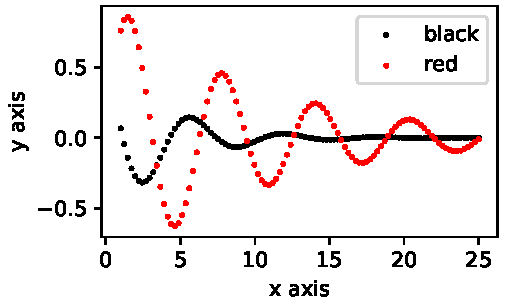
\includegraphics{vector_scatter}
	\caption{Example of a vector image with scattered point.}
	\label{vector_scatter}
\end{figure}

\section{Raster images}
\lipsum[1]

\begin{figure}
	\centering
	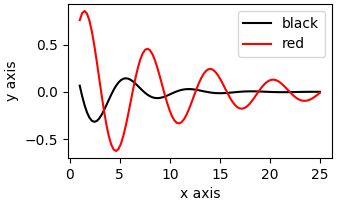
\includegraphics{raster_solid}
	\caption{Example of a raster image with solid lines.}
	\label{vector_solid}
\end{figure}

\lipsum[2]

\begin{figure}
	\centering
	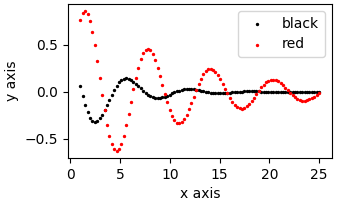
\includegraphics{raster_scatter}
	\caption{Example of a raster image with scattered point.}
	\label{vector_scatter}
\end{figure}

%Bibliography==============================

% \bibliography{Co3O2BO3_references}

\end{document}
